\documentclass[letterpaper]{article}

\usepackage{aaai}
\usepackage{amsmath}
\usepackage{amssymb}
\usepackage{amsthm}
\usepackage{courier}
\usepackage{graphicx}
\usepackage{helvet}
\usepackage{times}
\usepackage{verbatim}

\newtheorem{definition}{Definition}
\newtheorem{example}{Example}
\newtheorem{formula}{Formula}
\newtheorem{problem}{Problem}

%\setlength\parindent{0pt}
\frenchspacing

\setlength{\pdfpagewidth}{8.5in}
\setlength{\pdfpageheight}{11in}

\newcommand{\bigsetdef}[2]{\big\{#1\,\,\big\vert\,\,#2\big\}}
\newcommand{\cardinality}[1]{\lvert#1\rvert}
\newcommand{\pair}[2]{\langle#1,#2\rangle}
\newcommand{\range}[2]{#1, \ldots, #2}
\newcommand{\set}[1]{\{#1\}}
\newcommand{\setdef}[2]{\{#1\,\vert\,#2\}}
\newcommand{\triple}[3]{\langle#1,#2,#3\rangle}
\newcommand{\tuple}[1]{\langle#1\rangle}

\pdfinfo{
/Title Rough Set Semantics for Identity on the Web
/Author Wouter Beek, Stefan Schlobach, Frank van Harmelen}
\setcounter{secnumdepth}{0}

\begin{document}

\title{Rough Set Semantics for Identity on the Web}
\author{Wouter Beek \and Stefan Schlobach \and Frank van Harmelen\\
Vrije Universiteit Amsterdam\\
De Boelelaan 1081a\\
1081HV Amsterdam\\
The Netherlands}
\maketitle
\begin{abstract}
\begin{quote}
Identity relations are at the foundation of the Linked Open Data initiative
  and on the Semantic Web in general.
They allow the interlinking of alternative descriptions of the same thing.
However, many practical uses of \verb|owl:sameAs| are known to violate its
  formal semantics.
We propose a method that assigns meaning to (the subrelations of)
  an identity relation using the predicates of the dataset schema.
Applications of this approach include automated suggestions for
  asserting/retracting identity pairs and quality assessment.
We also describe an experimental design for this approach.
\end{quote}
\end{abstract}

\section{Introduction}
\label{sec:introduction}

Identity relations are at the foundation of the Linked Open Data initiative
  and of the Semantic Web in general \cite{bizer_cyganiak_heath_2007}.
They allow the interlinking of alternative descriptions of the same thing.
However, the traditional notion of identity
  (expressed by \verb|owl:sameAs| \cite{motic_paterschneider_grau_2012})
  is often problematic, e.g. when objects are considered the same in some
  contexts but not in others.
The standing practice in such cases is to use weaker relations of relatedness
  (e.g., \verb|skos:related|).
Unfortunately, this limits reasoners in drawing inferences.

According to the traditional semantics of the identity relation,
  identical terms can be replaced for one another in all non-modal contexts
  \emph{salva veritate}.
Practical uses of \verb|owl:sameAs| are known to violate this strict condition
  \cite{halpin_hayes_2010,halpin_hayes_mccusker_mcguinness_thompson_2010}.

\subsection{Previous work}
\label{sec:previous_work}

Existing research proposes the following solutions for the problem of
  identity relations on the Semantic Web.
(1) Introduce weaker versions of \verb|owl:sameAs|
  \cite{halpin_hayes_2010,mccusker_mcguinness_2010}
  (e.g., \verb|skos:related|).
(2) Restrict the applicability of identity relations to specific contexts.
  Identities are expected to hold within a named graph or within a namespace,
  but not necessarily outside of it \cite{halpin_hayes_2010,melo_2013}.
(3) Introduce additional vocabulary that does not weaken but extend
  the existing identity relation \cite{halpin_hayes_2010}.
  For example, allow an explicit distinction to be made between mentioning
  a term and using a term
  (e.g., a car and a Web document describing that car).
(4) Add domain-specific weaker versions of the identity relation
  \cite{mccusker_mcguinness_2010} (e.g., ``have the same medical use''
  is weaker than ``are the same molecule'').
(5) Adapt the modeling practice, possibly in a (semi-)automated way
  by adapting visualization and modeling toolkits to produce notifications
  upon reading SW data, or by posing additional restrictions on the creation
  and alteration of data. For example adding an RDF link could require
  reciprocal confirmation from the maintainers of the respective datasets.
  \cite{halpin_hayes_2010,ding_shinavier_finin_mcguinness_2010}

Other related research focusses on the extraction of network properties of
  \verb|owl:sameAs| datasets \cite{ding_shinavier_shangguan_mcguinness_2010},
  but these endeavors are not yet related to the semantics of the
  identity relation.

What these approaches have is common is that quite some work has to be done
  (adapting or creating standards, instructing modelers, converting existing
  dataset) in order to resolve some of the problems of identity.
Our approach provides a way of dealing with the heterogeneous real-world usage
  of identity in the Semantic Web that is fully automated and that requires
  no changes to standards, modeling practices, or existing datasets.

\subsection{Research goals}
\label{sec:research_goals}

In developing our approach we have the following research goals:
\begin{enumerate}
\item In an identity relation the pairs all look the same.
      We want to characterize subrelations of an identity relation in terms
      of the predicates that occur in the schema of the dataset.
\item Based on an existing identity relation we want to give semantically
      motivated suggestions for extending/limiting the identity relation.
\item We want to assess the quality of an identity relation based on
      the consistency with which it is applied to the data.
\end{enumerate}

\section{Approach}
\label{sec:approach}

In the following we consider an arbitrary,
  materialized RDF graph $G$ and an identity relation $\sim$ over
  the resources that occur in $G$.
The subject terms of $G$ are denoted by $S_G$, the predicate terms by $P_G$
  and the object terms by $O_G$.

For illustrative purposes we use the IIMB dataset that is used in the
  instance matching track of the 2012 Ontology Alignment Evaluation
  Initiative (OAEI) \cite{oaei_2012}.
This dataset consists of eighty ontologies $G_i$ (for $1 \leq i \leq 80$)
  that are linked to a single base ontology $G_0$.
A graph $G$ is the result of fully materializing the graph merge
  of $G_i$ (for some $1 \leq i \leq 80$) and $G_0$.
For each of these eighty linked ontologies a reference mapping is available.

In RDF a property consists of a single predicate term
  (e.g., the property ``is spoken in'' is denoted by predicate term
   \verb|IIMBTBOX:spoken_in| in the IIMB dataset).
We generalize the notion of a property to consist of
  an arbitrary number of predicate terms.
For this we define a depth-$n$ \emph{predicate path map} (abbr. ppm)
  that is characterized by a sequence of $n$ predicates
  and denotes a (functional) mapping from subject terms
  into sets of object terms
  (def. \ref{def:predicate_path},
   where $p_i \in P_G$ and $[p]_{\sim}$ is the identity set for $p$).
%$f_{\tuple{\range{p_1}{p_n}}}: S_G \rightarrow \mathcal{P}(O_G)$

\small
\begin{definition}[Predicate path map (ppm)]
\begin{align}
\label{def:predicate_path}
  f_{\tuple{\range{p_1}{p_n}}}(s)
\,=\,
  \bigsetdef{o \in O_G}{
    \exists_{\range{x_1}{x_{n-1}}} \quad \quad \quad \quad \quad \quad\\
      \bigwedge_{i=0}^{n-1}\nolimits
          \pair{I(x_i)}{I(x_{i-1})}
        \in
          \bigcup_{p \in [p_{i+1}]_{\sim}}\nolimits \mathit{Ext}(I(p))
  }\nonumber
\end{align}
\end{definition}
\normalsize

\noindent Examples of properties characterized by predicate path maps are
  ``is spoken in'' (depth-$1$) and
  ``is spoken in a country whose form of government is'' (depth-$2$).

\subsection{Shared properties and indiscernibility}
\label{sec:indiscernibility}

When we look at the triples that constitute a set of identity relations,
  we see that all links look the same.
But when we take the triples in which the subject and object terms occur
  into account, we see that within the identity relation there may be
  different subrelations that we can identify in terms of the predicates
  that occur in the schema.

For instance, in the IIMB dataset there are some identical resources that
  share the property \verb|IIMBTBOX:spoken_in|, while other pairs share
  the property \verb|IIMBTBOX:form_of_government|.
The set of pairs of resources that are spoken in the same language may even
  be disjoint from the set of pairs of resources that have the same
  form of government.

Note that we are not only interested in the properties that resources share
  with one other (e.g., where they are spoken, or which form of government
  they have), but we are also interested in resource pairs that share
  the same sharing properties.
We can thus identify subsets of an identity relation based on differences
  in the sets of predicate path maps relative to which they take resources
  to be \emph{indiscernible} from one another.

In the example above, one subset of the identity relation does not discern
  resources that are spoken in the same language, whereas another subset
  of the identity relation does not discern resources that have the same
  form of government.

We say that two resources are indiscernible with respect to
  a set of predicate path maps $P \subset P_G^n$
  in case they share the same properties denoted by those ppms
  (def. \ref{def:resource_indiscernability}).\footnote{
    $P$ must be closed under the identity relation, i.e.,
    \begin{equation*}
      cl_{\sim}(P) = \bigcup_{\tuple{\range{p_1}{p_n}} \in P}\nolimits (
        [p_1]_{\sim} \times \ldots \times [p_n]_{\sim}
      )
    \end{equation*}}
We say that two resource pairs are indiscernible
  in case both pairs are indiscernible for the same
  $P^* \subseteq \mathcal{P}(P_G^n)$
  (def. \ref{pair indiscernibility}).\footnote{
    In order to assertain that $f_p(x)$ and $f_p(y)$ denote
      the same set of resources, identity does not suffice.
      $\approx$ gives a special treatment for blank nodes and
      typed literals (skipped here for brevity).
  }

\small
\begin{definition}[Indiscernibility]
\begin{align}
\label{def:resource_indiscernability}
\mathit{IND}(P) \,=\,
  \setdef{
    \pair{x}{y} \in S_G^2
  }{
    \forall_{p \in cl_{\sim}(P)} f_p(x) \approx f_p(y)
  }
\\
\label{pair indiscernibility}
\mathit{IND}(P^*) \,=\,
  \setdef{
    \pair{\pair{x_1}{y_1}}{\pair{x_2}{y_2}} \in (S_G^2)^2
  }{\\
    \forall_{P \in P^*}
        \pair{x_1}{y_1} \in \mathit{IND}(P)
      \leftrightarrow 
        \pair{x_2}{y_2} \in \mathit{IND}(P)
  }\nonumber
\end{align}
\end{definition}
\normalsize

\noindent As explained above, for a given set of identity pairs there
  may be multiple pairs that have the same shared properties.
These sets of predicates that are shared across resource pairs are
  considered to give a description of a specific subrelation of
  the identity relation.

According to the standard definition,
  identical resources are indiscernible with respect to all properties.
We take a given set of identity pairs and partition it into subsets which
  we can describe as being $cl_{\sim}(P)$-indiscernible,
  for $P \subseteq P_G^n$.

Fig. 1 shows an example
  of a discernibility partitioning for a given identity relation.

\begin{figure*}
\label{fig:iimb_example}
\centering
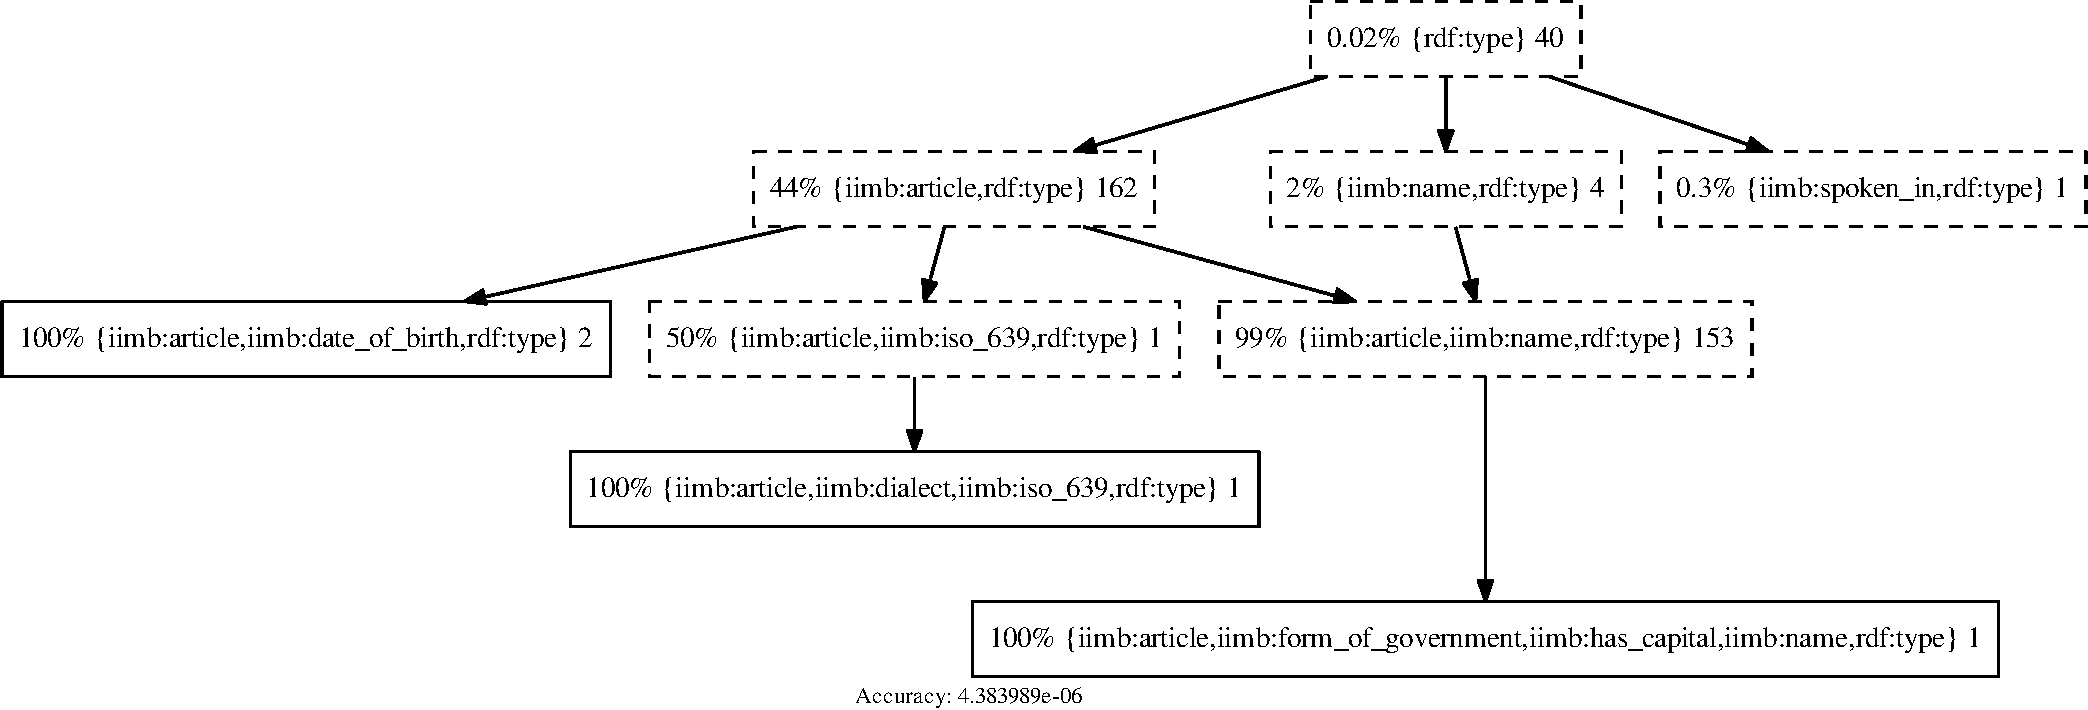
\includegraphics[width=\textwidth]{iimb_approximation_example_crop}
\caption{
  An example of a discernibility partition for an identity relation
    consisting of 365 pairs applied to the fourth IIMB linkset.
  Each node is annotated with the set of predicates $P$ for which
    its pairs are $P$-indiscernible.
  The number of identity pairs within each partition set
    is displayed to the right of the predicate set label.
  Partition sets that contain no identity pair are not show.
  The number that occurs to the left of the predicate label in each node
    indicates how may pairs in that node are identity pairs.
  The lower approximation consists of the nodes with a solid border,
    indicating that they contain only identity pairs.
  The higher approximation consists of all displayed nodes.}
\end{figure*}

\subsection{Approximation}
\label{sec:approximation}

In the previous section we partitioned a given identity relation $\sim$
  into subrelations that can be distinguished in terms of schema predicates
  (or $n$-depth paths of those predicates).
In this section we create an approximation of the identity relation.
This approximation will allow us to
  (1) give suggestions about which pairs to in/exclude from
      the identity relation, and
  (2) give an indicator for the quality of the identity relation.

For the approximation of the identity relation we use
  rough set theory \cite{pawlak_1991} to represent an approximation of
  a given identity relation $\sim$.
The domain for our rough set approach is the Cartesian product of $S_G$.
The set of predicates is the powerset of $P_G$.
%\footnote{
%  Relations are called `attributes' in rough set theory.
%  They are functions that map to an arbitrary set of value labels.
%  We only consider functions that map from binary input into
%    the set of Boolean truth values, and therefore use the term
%    `predicates' to denote these functions.
%}
%This means that we have a big number of primitives to work with
%  (quadratic in the number of constants;
%   exponential in the number of relations).

For an arbitrary binary relation $\sim$ we can define
  a higher (def. \ref{def:higher_approximation}) and
  a lower (def. \ref{def:lower_approximation}) approximation
  of that relation.
In definitions \ref{def:higher_approximation} and
  \ref{def:lower_approximation},
  $\mathbb{R}$ characterizes a similarity relation between resource pairs.
The intuition behind these definitions is that non-$\sim$-pairs
  that are similar to $\sim$-pairs should be in the higher approximation,
  whereas no $\sim$-pair that has a similar non-$\sim$-pair should be
  in the lower approximation.

\small
\begin{definition}[Higher \& lower approximation]
\begin{align}
\label{def:higher_approximation}
x \overline{\sim} y \, & \iff & \,
  \exists u,v (\pair{u}{v} \mathbb{R} \pair{x}{y} \,\land\, u \sim v)
\\
\label{def:lower_approximation}
x \underline{\sim} y \, & \iff & \,
  \forall u,v (\pair{u}{v} \mathbb{R} \pair{x}{y} \,\rightarrow\, u \sim v)
\end{align}
\end{definition}
\normalsize 

\begin{comment}
\small
\begin{definition}[Higher \& lower approximation]
\label{def:higher_lower_approximation}
\begin{align}
  y \in [x]_H
\,\iff\,\\
  \exists u (
      \cardinality{[u]_{\sim}}>1
    \,\land\,
      \mathbb{P}([u]_{\sim})=\mathbb{P}(\set{x,y})
  )\nonumber
\\
  y \in [x]_L
\,\iff\,
  \forall S \subseteq D (\\
      (\cardinality{S}>1 \,\land\, \mathbb{P}(S) = \mathbb{P}(\set{x,y}))
    \,\rightarrow\,
      \exists s \in D (S=[s]_{\sim})
  )\nonumber
\end{align}
\end{definition}
\normalsize
\end{comment}

\noindent Since we want to stay close to the traditional notion of identity,
  defined in terms of indiscernibility,
  we choose $\mathit{IND}(\mathcal{P}(P_G^n))$ as our similarity relation.

Figure 1 shows an example of the lower and higher
  approximations for a linkset.
Since in this figure a partition is only drawn when there is at least one
  identity pair that is indiscernible with respect to some set of
  predicates, the higher approximation amounts to the entire figure.
The lower approximation only consists of those partition sets that contain
  at least one identity pair, and that contain no non-identity pair.

\subsection{Quality}
\label{sec:quality}

Given the rough set representation $\pair{\underline{\sim}}{\overline{\sim}}$
  of identity relation $\sim$, we can calculate the accuracy of this
  approximation with equation \ref{eq:accuracy}.

\small
\begin{equation}
\label{eq:accuracy}
  \alpha(\sim)
\,=\,
  \cardinality{\underline{\sim}} / {\cardinality{\overline{\sim}}}
  %\dfrac{\cardinality{\underline{\sim}}}{\cardinality{\overline{\sim}}}
\end{equation}
\normalsize

The intuition behind the usefulness of equation \ref{eq:accuracy}
  is that the crispness of a set should be proportional to the quality
  of the identity relation on which it is based.
Since a consistently applied identity relation has relatively many
  partition sets that contain either
  no identity pairs (small value for $\overline{\sim}$) or
  only identity pairs (big value for $\underline{\sim}$),
  a more consistent identity relation has a higher accuracy.

Now that we have a formal metric for identity relation quality,
  we can define the characteristics of an ideal identity relation.
Traditionally the ideal identity relation ensures indiscernibility
  for all expressible properties in the language
  (the principle of the indiscernibility of identicals).
According to this traditional view an identity relation becomes of
  higher quality by considering more predicates (or ppms)
  according to which two resources are not allowed to be discernible.
We give a different quality criterion.

We observe that for a given equivalence relation $\sim$
  defined over a domain of resources $S_G$ we can define the notion of
  full discernibility:

\small
\begin{definition}[Discernible model]
\label{def:fully_discernible}
\begin{align}
& \text{A domain $S_G$ is fully discernible w.r.t. a binary relation $\sim$ iff}
\nonumber
\\
 & \forall x,y \in S_G (
    [x]_{\sim}=[y]_{\sim}
  \,\lor\,\,
    \mathbb{P}([x]_{\sim}) \neq \mathbb{P}([y]_{\sim})
  )
\end{align}
\end{definition}
\normalsize

\noindent From this definition it is clear that a domain of discourse
  is fully discernable just in case there exists a binary relation $\sim$
  such that \mbox{$\alpha(\sim) = 1.0$}.

\section{Experimental design}
\label{sec:experimental_design}

In section \ref{sec:research_goals} we enumerated three research goals.
The first goal is met, since an indiscernibility partition characterizes
  subrelations based on the ppms $P$ for which the pairs in that sets
  are $cl_{\sim}(P)$-indiscernible.
In this way we can distinguish between different types of identity
  by treating $P$ as a description of a (sub)set of identity pairs.

The second goal is met, since the notion of a rough set allows us to
  distinguish between pairs that must be (lower approximation)
  and those that may be (i.e., ``not must not'', higher approximation)
  in the identity relation.
If we want to add/remove pairs of the identity relation,
  we should not consider pairs of the former but only pairs of
  the latter kind.

The third goal is met, since the measure for rough set accuracy
  is based on the discernibility criteria of an identity set.
The crispness of the set is proportional to the quality of the
  identity relation, based on its semantic consistency.

Our approach provides a new experimental design for evaluating
  hypothesis regarding identity relations that have not been
  evaluated before in terms of the semantics of the data.

\subsection{Hypotheses}
\label{sec:hypotheses}

Using this new approach the following hypothesis can be validated:

\begin{enumerate}
\item Take an \verb|owl:sameAs| relation and a \verb|skos:related|
        relation defined over the same domain.
      Merge them into a new binary relation $\sim$.
      Establishing the lower and higher approximation of $\sim$,
        the hypothesis is that pairs from \verb|owl:sameAs| occur more
        frequently in the lower boundary than pairs from \verb|skos:related|.
\item Take a set of alignment pairs, each of which is associated with
        a confidence measure between $0.0$ and $1.0$.
      Choose an arbitrary cutoff point $0.0<c<1.0$.
      The hypothesis is that alignments with a confidence larger than $c$
        occur more frequently in the lower approximation than alignments
        with a confidence smaller than $c$.
\item Take a set of automatically generated alignment pairs with
        associated confidence measures and take the gold standard or
        reference alignment for the same dataset.
      The hypothesis is that pairs that occur in the lower approximation
        of the alignment appear relatively more often in the gold standard
        than pairs that occur in the higher approximation of the alignment.
\item The accuracy measure $\alpha$ of a reference alignment is generally
        higher than the accuracy measure of an automatically generated
        alignment for the same dataset.
      Or, the accuracy measure is generally higher for identity relations
        that are considered correct by domain experts.
\end{enumerate}

\subsection{Implementation}
\label{sec:implementation}

The implementation built for this paper is deployed as an extension pack
  of the ClioPatria triple store \cite{schreiber_2006}.
For RDF graphs that are loaded in ClioPatria this extension calculates
  the discernibility partition, rough set approximation and accuracy.
The results are visualized using GraphViz and are displayed in a
  Web interface using SVG.
Interactive Ajax code allows the user to click on nodes in the SVG graphic
  to navigate to descriptions of the resource pairs that occur in
  that partition set while not being in the identity relation.
This implementation may facilitate the validation of hypotheses in this
  new experimental setup.

\section{Conclusion}
\label{sec:conclusion}

In this paper we have given an new approach for characterizing,
  extending/retracting, and assessing identity relations.
Our approach does this in purely qualitative terms, using schema semantics.
In contemporary ontology alignment and data linking activities nonsemantic
  aspects of resources play a role as well.
For instance similarity assessment for natural language labels is often
  used in data linking.

We think that the qualitative means of characterizing an identity relation
  are a useful addition to existing quantitative means.
Also, we think that it is more useful and viable to enrich existing
  identity relations in the LOD based on the semantics of the datasets
  in which they occur, than to introduce new relationships into SW languages.
Apart from the practical difficulties of teaching practitioners
  and transforming/enriching existing datasets, we suggest that the
  meaning of an identity (sub)relation is partially defined in its use,
  i.e., in the indiscernibility criteria it embodies.

For our approach it is not necessary to pose additional restrictions
  on a binary relation $\sim$.
The definitions in this paper apply to \verb|owl:sameAs| relations
  in the same way in which they apply to any other binary relation
  (e.g., \verb|skos:related|).

We are currently in the process of validating the above enumerated hypotheses.
The results of these evaluations are continuously being published on
  \verb|wouterbeek.com/identity-on-the-web|.
The website currently contains the automated results of all eighty IIMB
  alignments, drawn from the instance matching track of the
  OAEI 2012.
The website also refers to the publicly available Git repository
  \verb|github.com/wouterbeek/IOTW| where the implementation
  discussed in section \ref{sec:implementation} can be found.

\bibliographystyle{aaai}
\bibliography{rough_set_semantics_for_identity_management_on_the_web}

\begin{comment}
For example, in figure \ref{fig:indiscernibility_example} the subrelation
  $\set{\pair{a}{c}, \pair{b}{c}}$ is characterized by
  $\mathcal{P}(\set{P})$.

\begin{figure}[h!]
\centering
\label{fig:indiscernibility_example}
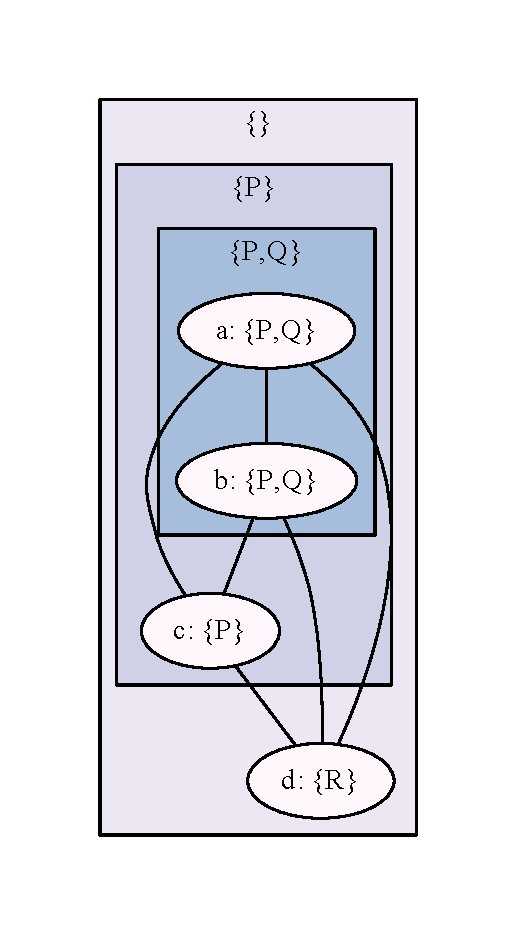
\includegraphics[scale=0.7]{indiscernibility_example}
\caption{
  This figure contains four resources, represented by nodes and
    annotated with the properties $P$, $Q$, and $R$ that apply to them.
  It also contains six pairs, represented as edges between the nodes
    (reflexive pairs are not shown).
  The edges are drawn inside squares that represent the indiscernibility
    sets to which they belong.
  For instance $\pair{a,c}$ and $\pair{a,c}$ belong to the same
    indiscernibility set $\set{P}$, but $\pair{a,b}$ belongs to
    indiscernibility set $\set{P,Q}$.}
\end{figure}
\end{comment}

\end{document}

